\documentclass{standalone}
\usepackage{tikz}
\usetikzlibrary{positioning, shapes}

\begin{document}
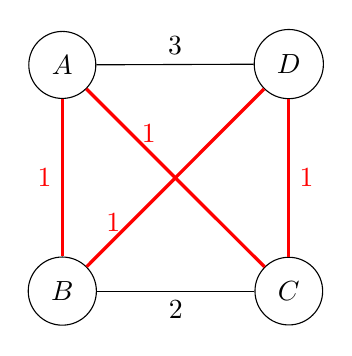
\begin{tikzpicture}[v/.style = {circle, draw, inner sep = 5pt}, 
	e/.style = {red, very thick},
	node distance = 2.0cm]
  \node (a) [v] {$A$};
  \node (b) [v, below = of a] {$B$};
  \node (c) [v, right = of b] {$C$};
  \node (d) [v, above = of c] {$D$};

  \draw[e] (a) to node[left] {1} (b);
  \draw (b) to node[below] {2} (c);
  \draw[e] (c) to node[right] {1} (d);
  \draw (d) to node[above] {3} (a);
  \draw[e] (a) to node[near start, right] {1} (c);
  \draw[e] (b) to node[near start, left] {1} (d);
\end{tikzpicture}
\end{document}
